\documentclass[titlepage, 12pt]{article}

\usepackage{framed}
\usepackage{enumitem}
\usepackage{geometry}
\geometry{
  letterpaper,
  margin=1in,
}

\usepackage{graphicx}
\graphicspath{{./images/}}
\usepackage{hyperref}
\usepackage{float}
% \usepackage{subcaption}
\usepackage{amssymb}

\title{SE 2XB3 Group 4 Report 9}
\author{
  Huang, Kehao \\
  400235182 \\
  \texttt{huangk53@mcmaster.ca} \\
  L01
  \and
  Jiao, Anhao \\
  400251837 \\
  \texttt{jiaoa3@mcmaster.ca} \\
  L01
  \and
  Ye, Xunzhou \\
  400268576 \\
  \texttt{yex33@mcmaster.ca} \\
  L01
}
\date{30 March 2021}

\begin{document}
\maketitle{}

\newpage{}

\section{Bellman-Ford Approximation}

Two versions of Bellman-Ford approximation are implemented. One is a direct
modification of the original Bellman-Ford implementation with a frequency map
which keeps track of the number of relaxation performed on each node. The other
version is our attempt to exploit the frequency map with the hope to exit the
function and return when all nodes are relaxed exactly \(k\) times. Figure
\ref{fig:rtcomp} and \ref{fig:tdcomp} are the results of experiments carried out
to evaluate the implementations on two metrics. The optimized version and the
original approximation operates in the same way in terms of how the distances
are computed. Therefore, Figure \ref{fig:tdcomp} only includes one total
distance for different approximation versions.
\begin{figure}[h]
  \centering
  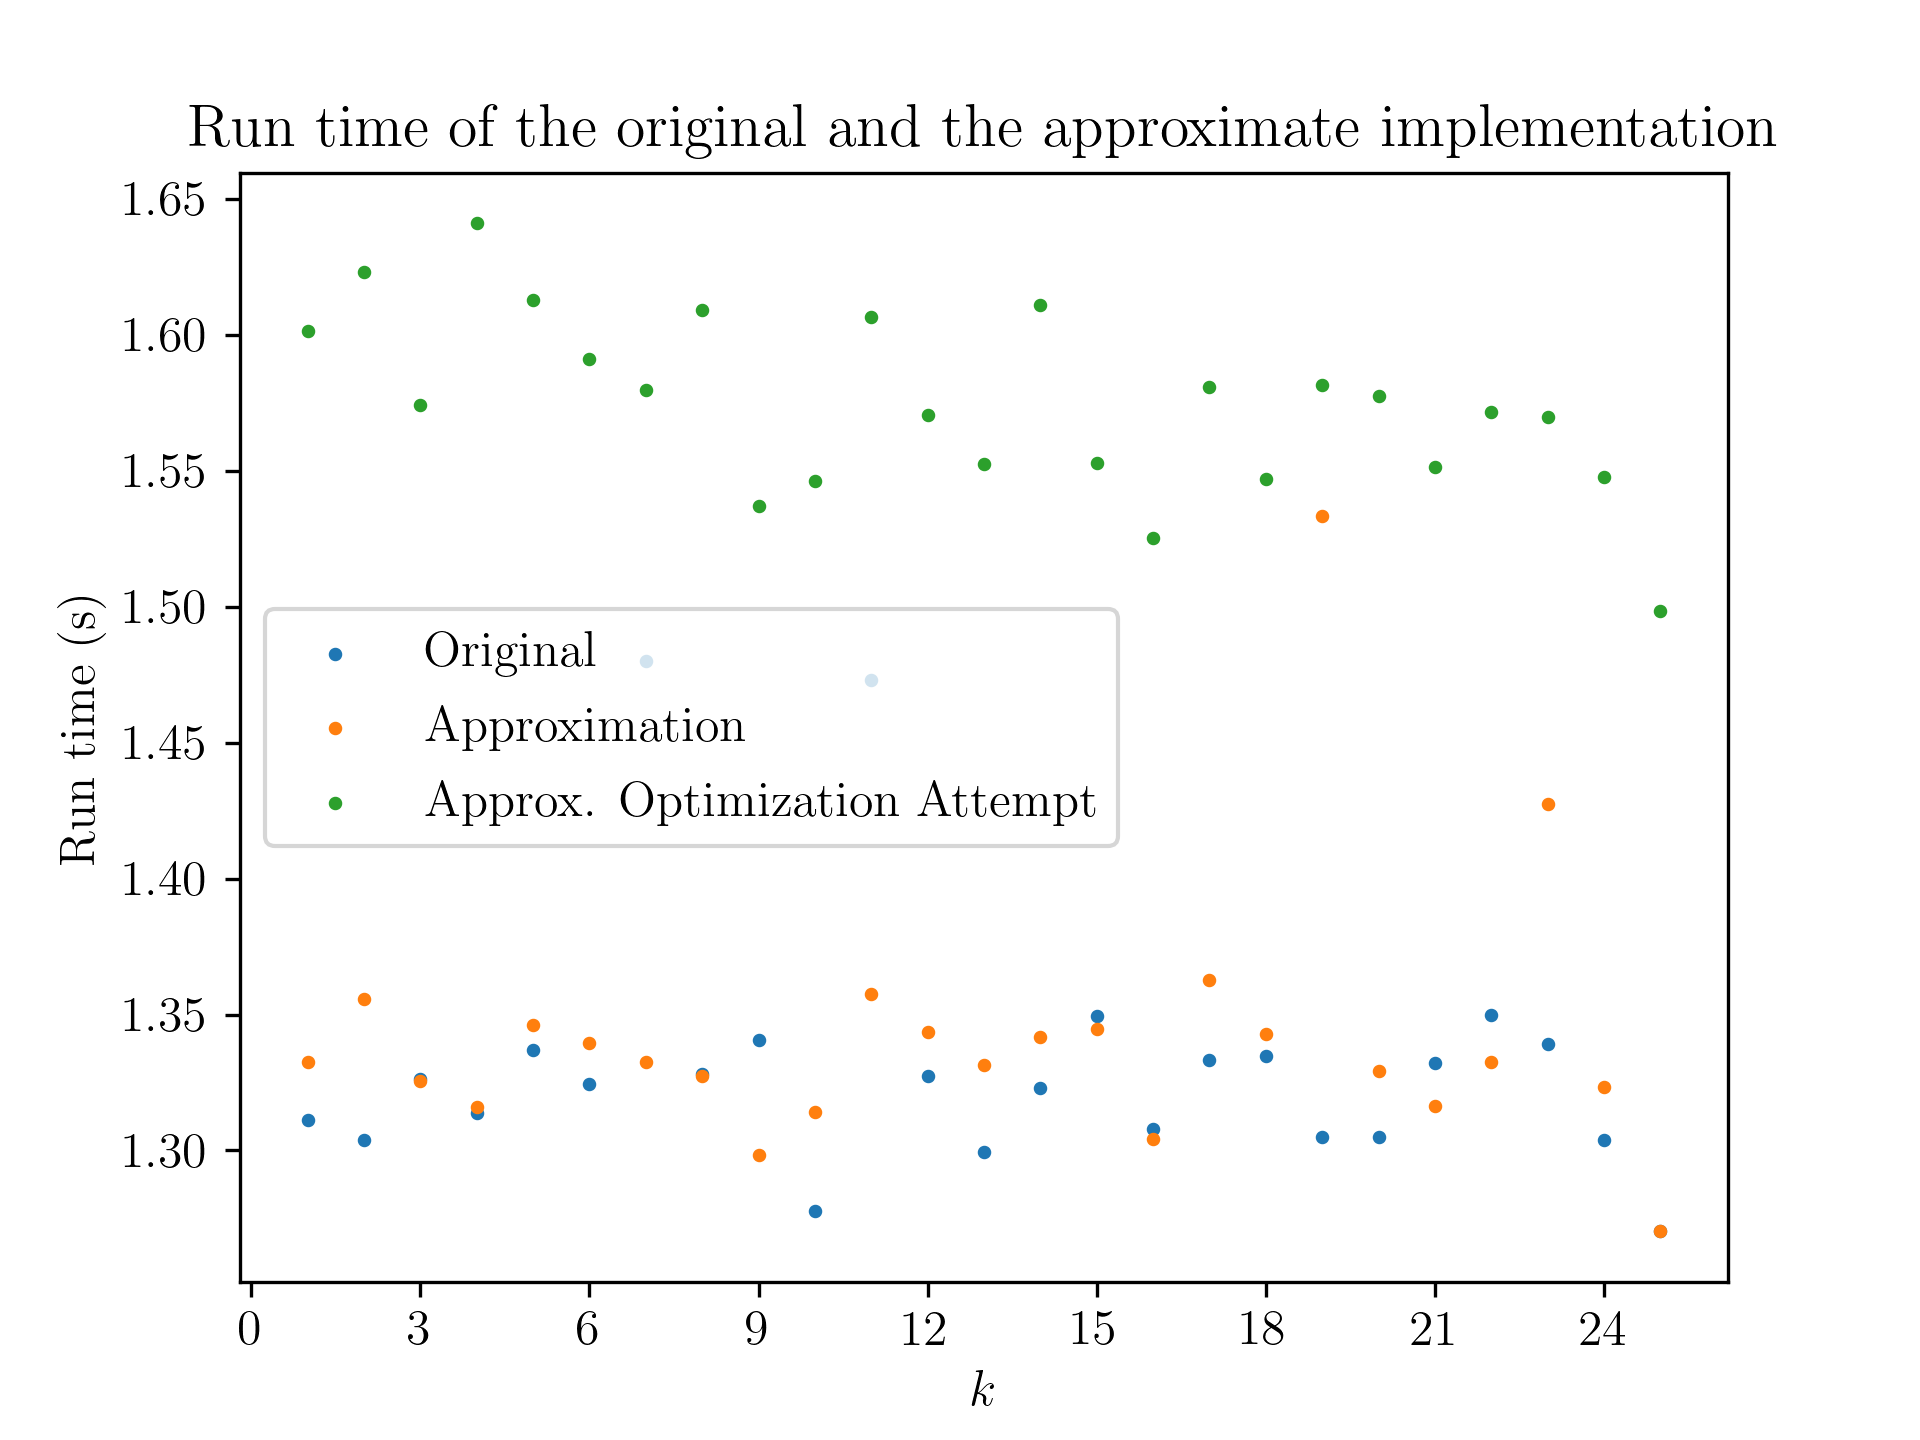
\includegraphics[width=0.8\linewidth]{rtcomp} 
  \caption{Run time comparison}
  \label{fig:rtcomp}
\end{figure}
\begin{figure}[h]
  \centering
  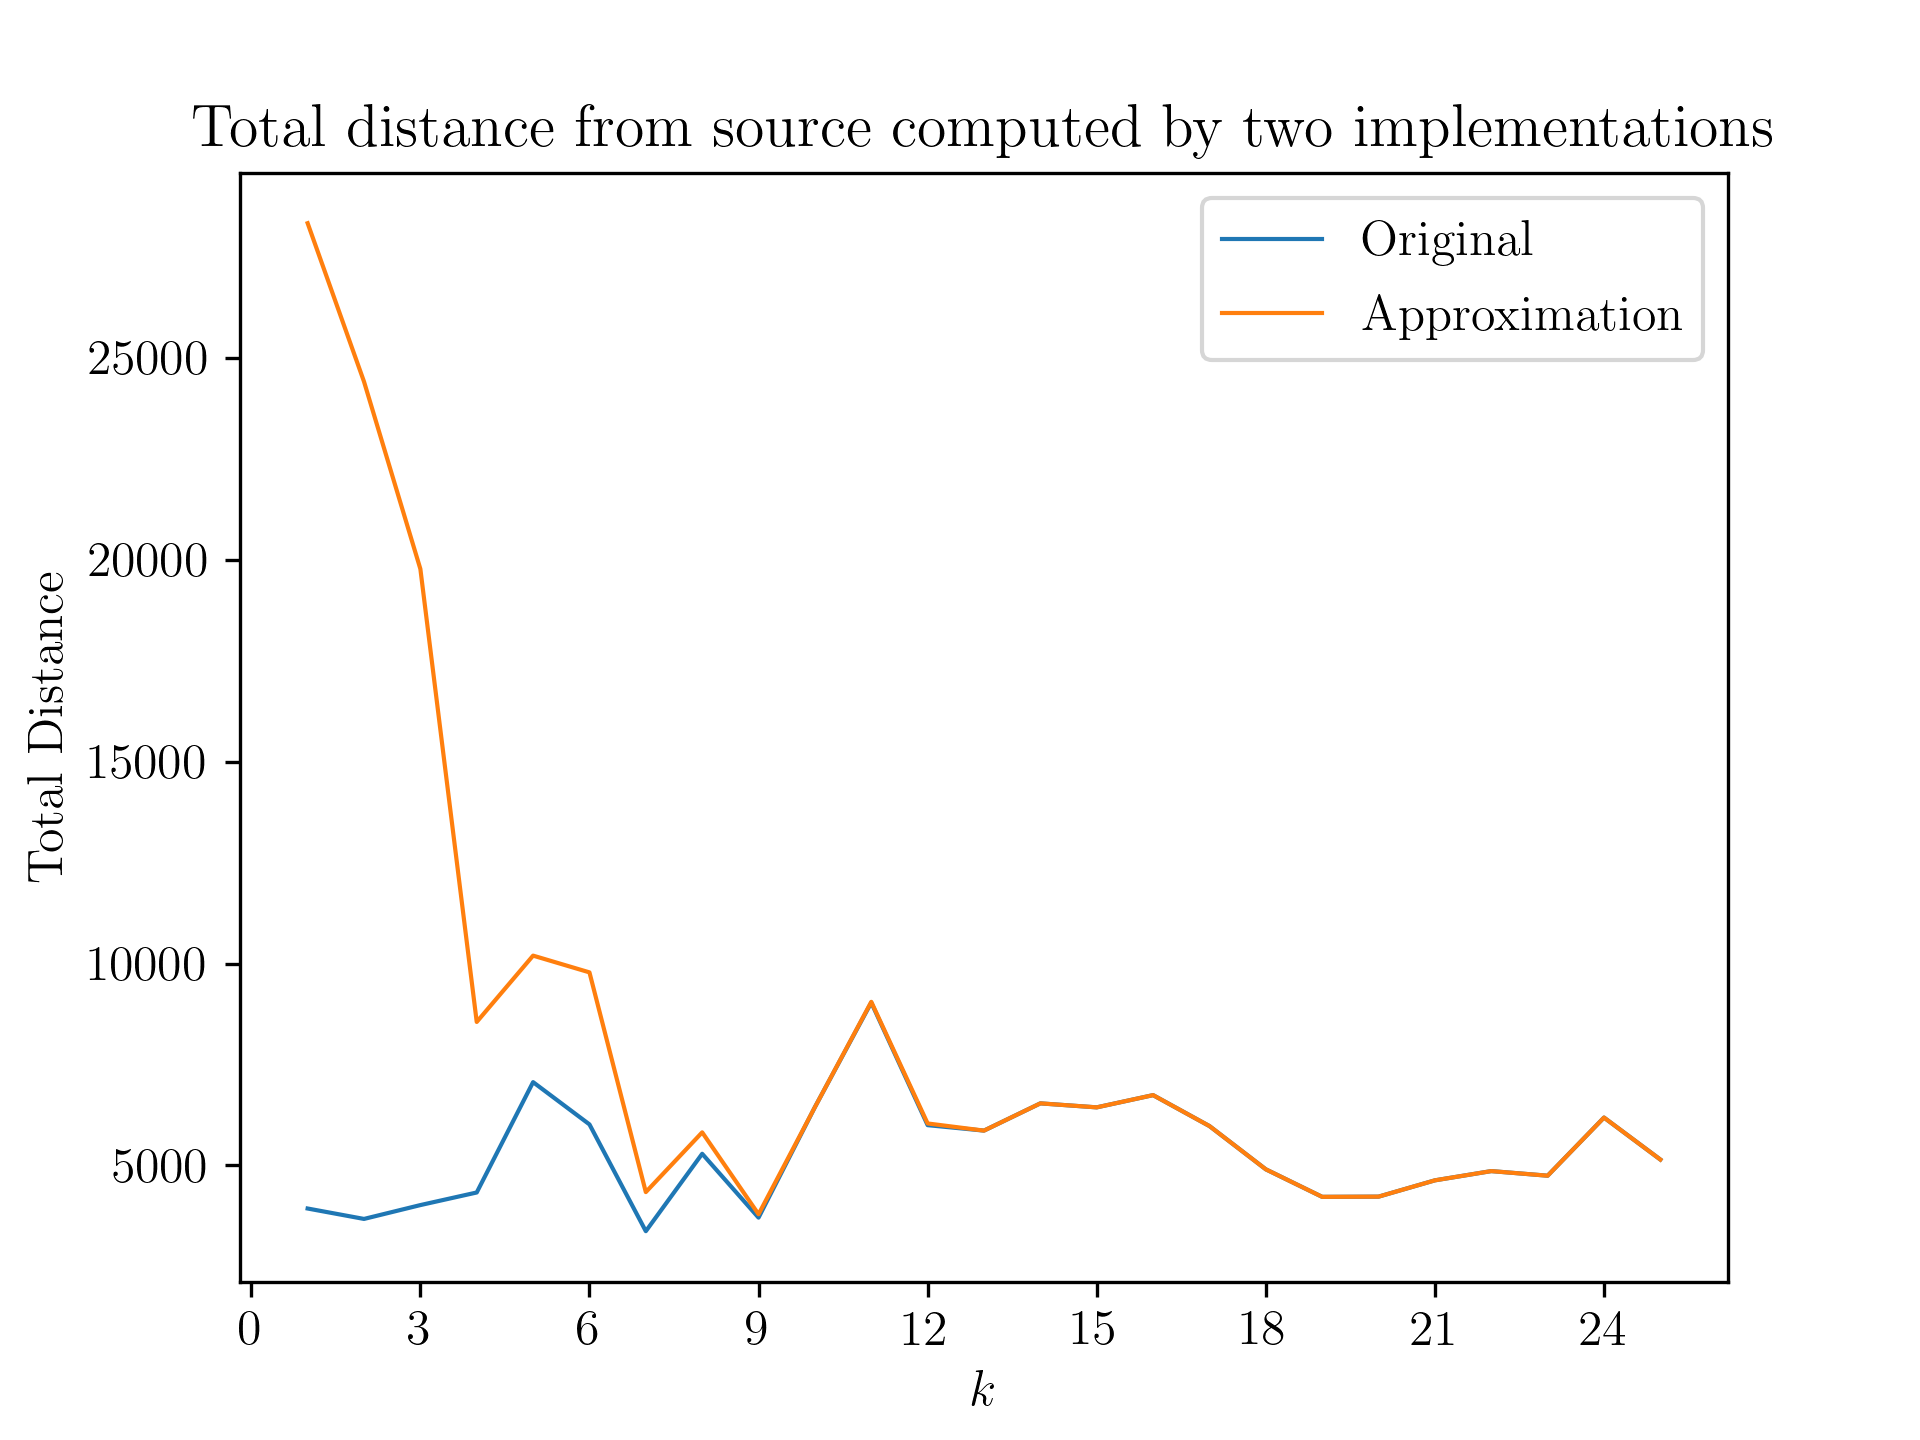
\includegraphics[width=0.8\linewidth]{tdcomp} 
  \caption{Total distance comparison}
  \label{fig:tdcomp}
\end{figure}

Surprisingly, our attempt for optimization is observably slower than the other,
while the difference in run time between the other two is insignificant. One
possible reason is that the extra \texttt{if} statement and \texttt{set}
operations introduced into the optimization attempt bring overheads to the
function. The time saved from breaking the loops is shorter than the time wasted
on processing the overheads.

Observing that in Figure \ref{fig:tdcomp}, the approximated total distance
merged with the accurate total distance computed by the original Bellman-Ford
implementation starting on \(k = 9\), the approximation implementation strictly
requires less relaxations in general. However, as indicated in Figure
\ref{fig:rtcomp}, the performance gain from the avoided relaxations is not
enough to make a consistent empirical difference. Considering that
approximations are not 100\% accurate, we propose that the original Bellman-Ford
implementation ensures the accuracy of the result and is overall the best among
the three.

\section{All Pairs Shortest Paths}

Our implementations of \texttt{all\_pairs\_dijkstra} and
\texttt{all\_pairs\_bellman\_ford} simply return the list of the results of
\texttt{dijkstra} and \texttt{bellman\_ford} called on every vertex. By knowing
the complexity of Dijkstra's and Bellman-Ford's algorithms are \(\Theta(V^2)\)
and \(\Theta(V^3)\), respectively, for dense graphs, calling the function for
\(V\) vertices results in the complexities of \(\Theta(V^3)\) for Dijkstra's and
\(\Theta(V^4)\) for Bellman-Ford's.

As for the \texttt{mystery} function, it is an implementation of Floyd's
algorithm. It finds the shortest paths between all pairs of the vertices. By
inspecting the code, the three nested \texttt{for} loops over the number of
vertices \(V\) confirm its time complexity of \(\Theta(V^3)\). After running
some small experiments with the implementation, we found that it can handle
graphs with negative edge weights. Given what the code does, the complexity is
not surprising because processing all possible pairs of vertices, or in another
word, filling the \(V \times V\) matrix itself is a \(\Theta(V^2)\) task. The
overall \(\Theta(V^3)\) complexity can be roughly perceived as taking
\(\Theta(V)\) time to process \(\Theta(V^2)\) pairs of vertices. In fact, Floyd's
algorithm can be understood as for any pair of vertices \(i\) and \(j\), try
every other node \(k\) to see if the path \(i \rightarrow k, k \rightarrow j\)
can improve the current path estimate \(i \rightarrow j\).

\end{document}
